\chapter{Wargame scenario}

Before launching the wargame, the user should be able to express agents and predefine agent behaviors. The user of the game should then be able to choose whether to use the predefined behavior, or take control of the agent himself. The user should also be able to define the behavior of an agent when it come close to other hostile agents. \\

\section{Rules}
These rules should apply to the wargame:
\begin{itemize}
	\item The game is turn-based. The turn end when the user is done executing commands, and press the \textit{End Turn} button.
	\item The game is played on a grid \ref{fig:ex_grid}.
	\item Each agent can move three grid-points in each turn.
	\item A higher ranked agent has a higher chance of winning.
	\item Agents fight when they are standing on the same grid location.
	\item The game rules are based on a classical deathmatch game. There is one winner only, and the winner is the team which eliminates all other team.
\end{itemize}

\begin{figure}[H]
\begin{center}
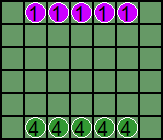
\includegraphics[scale=0.9]{Images/ex_grid.png}
\end{center}
\caption{Example of the grid setup with two opposing teams}
\label{fig:ex_grid}
\end{figure}

To get an overview of how the game operates, the layout of a game round is added in psuedocode.

\begin{source}{Game Round}{}
function gameRound()
{
	gameFrame();
	EndTurn();
}
\end{source}

The two functions called in the gameRound function, can be seen below.

\begin{source}{Game Frame}{}
for(i = 0; i <= 3; i = i + 1)
{
	CheckForEncounters();
	RandomAgentMovement();
	
	//Check if the list is empty
	if(moveAgents contains no items)
		return;
		
	UpdateAgentPositions();
	
	CheckForAgentCollisions();
}

\end{source}

The CheckForEncounters function will check if any of an agent is encountering, is within the reach of, another agent.
\begin{source}{Check for encounters}{}
foreach(agent a in agents)
{
	if(a is within bounderies of another agent)
	{
		a.RemoveAllMovements();
		a.encounter.Compile();
	}
}
\end{source}

If the current agent has no movements in his movement list, he finds a random agent from another team, and moves to their current location.
\begin{source}{Random agent movement}{}
foreach(agent a in agents)
{
	if(a has no movement)
	{
		agent moveToAgent = getRandomAgent();
		a.MoveToAgent(moveToAgent);
	}
}
\end{source}

The UpdateAgentPosistions function calculate the next agent move, taken from the moveAgents list. If the agent is still inside the warzone he can be moved. If the agent has reached his location his move gets removed from the list.
\begin{source}{Update agent positions}{}
foreach(agent a in agents)
{
	if(a.team == currentteam)
	{
		foreach(agent moveAgent in moveAgents)
		{
			a.CalculateNextPosition();
			if(a.NextPosition.IsInBounds())
			{
				a.MoveAgent();
			}
			if(a.IsAtEndPosition())
			{
				moveAgents.Remove(a);
			}
		}
	}
}
\end{source}

The CheckForAgentCollisions function will check if any agents from diffrent teams are standing on top of each other. If they happen to do so they will roll for the highest value, using their rank as a factor, to get the outcome of the fight. The agent with the lowest rolled value dies.
\begin{source}{Check for agent collisions}{}
for(agentCount = 0; agentCount < agnets.TotalAgents; agentCount++)
{
	foreach(agent a in agents)
	{
		if(a.CollideWithAgentOnOtherTeam())
		{
			if(a.Roll > CollidedAgent.Roll)
			{
				agents.Remove(CollidedAgent);
			}
			else
			{
				agents.Remove(a);
			}
		}
	}
}
\end{source}

The EndTurn function will check if any of the teams, as the only team, has agents left, which will result in a win for the current team. If there are no teams standing alone on the warzone, the turn is passed on to the next team.
\begin{source}{End turn}{}
if(only team 1 has agents)
{
	Team 1 wins!
}

...

else if(only team n has agents)
{
	Team n wins!
}

else
{
	switchTurn();
}
\end{source}